\documentclass[11pt]{article} 

\usepackage[top=1in,bottom=1in,left=1.5in,right=1.5in]{geometry} 

\usepackage{graphicx, soul, tikz, hyperref} 
\usepackage{amsfonts}
\usepackage{cases}
\usepackage{cleveref}
\usepackage{algorithm}
\usepackage{algpseudocode}
\usepackage{graphicx}
\usepackage{subcaption}

\newtheorem{reqn}{Requirement}

\begin{document} 

\thispagestyle{empty} 

\newgeometry{top=0.5cm, bottom=0.5cm, left=0.5cm,right=0.5cm} 

\begin{figure}[h] 

\centering 

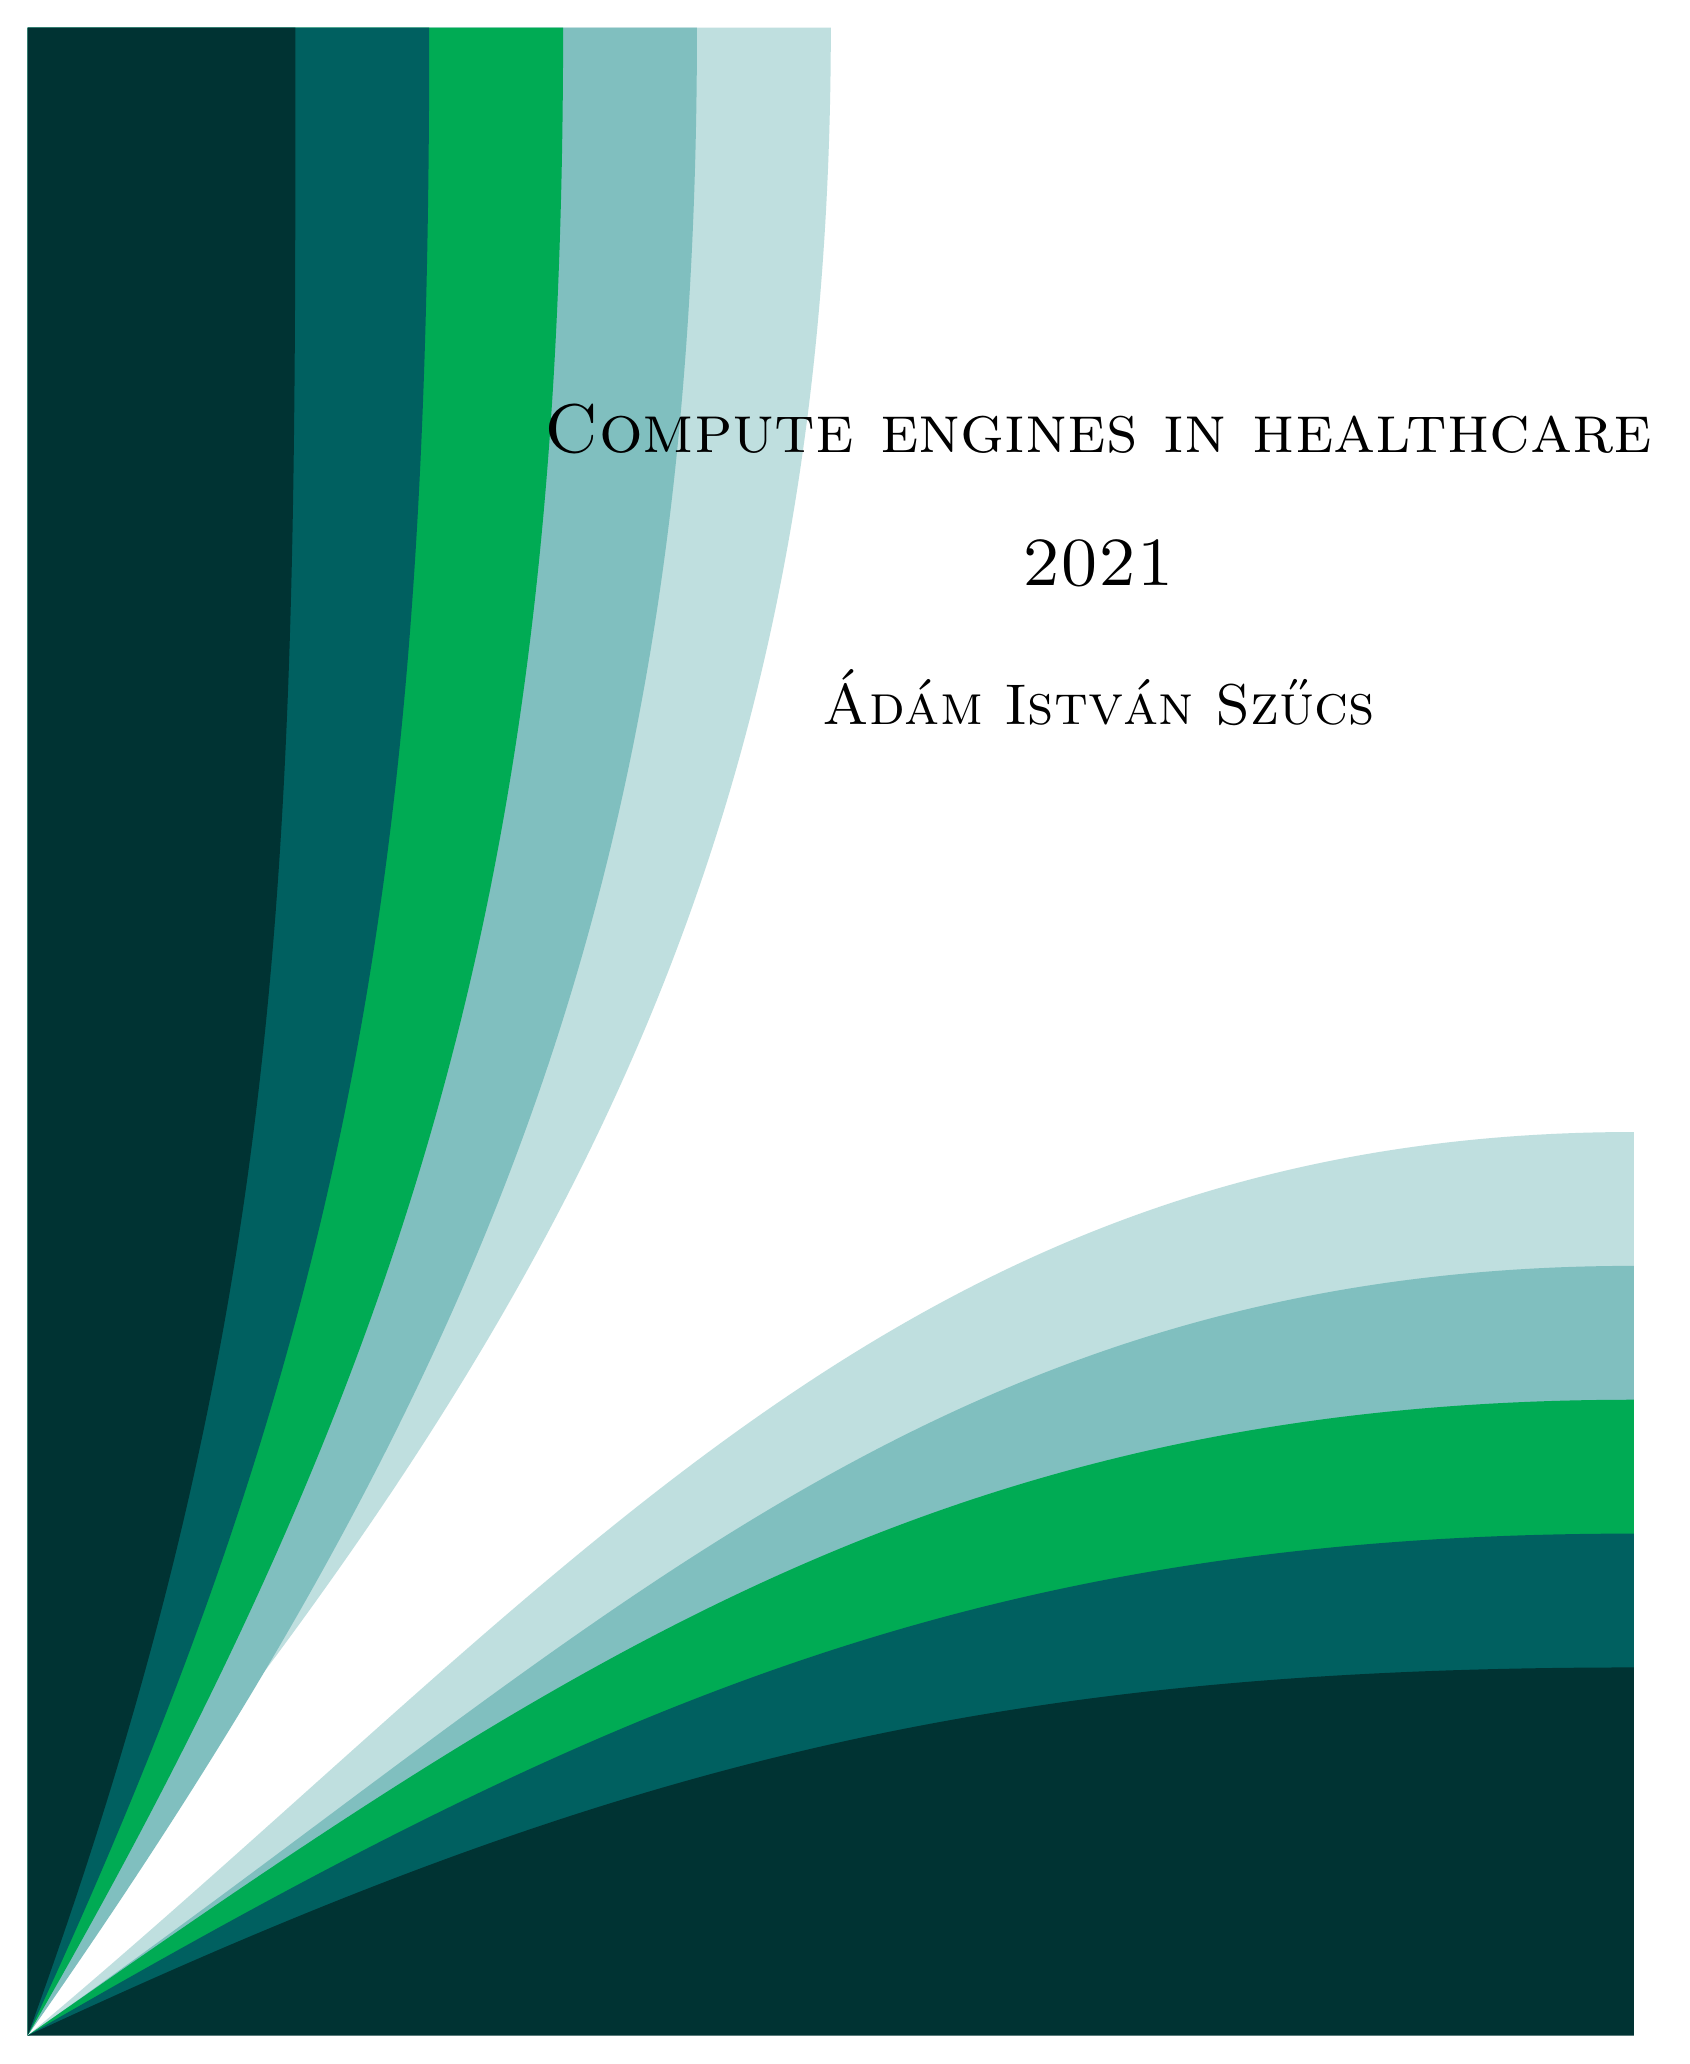
\begin{tikzpicture}[scale=0.85] 

\path[fill=white] (-10,-20) to [out=45,in=270] (4,10) -- (-10,10); 

\path[fill=white!75!teal] (-10,-19) to[out=50,in=270] (2,10) -- (-10,10); 

\path[fill=white!50!teal] (-10,-20) to[out=55,in=270] (0,10) -- (-10,10); 

\path[fill=green!67!blue] (-10,-20) to[out=60,in=270] (-2,10) -- (-10,10); 

\path[fill=teal!75!black] (-10,-20) to[out=65,in=270] (-4,10) -- (-10,10); 

\path[fill=black!60!teal] (-10,-20) to[out=70,in=270] (-6,10) -- (-10,10); 

\path[fill=white] (-10,-20) to[out=45,in=180] (14,-4.5) -- (14,-15); 

\path[fill=white!75!teal] (-10,-20) to[out=40,in=180] (14,-6.5) -- (14,-15); 

\path[fill=white!50!teal] (-10,-20) to[out=35,in=180] (14,-8.5) -- (14,-15); 

\path[fill=green!67!blue] (-10,-20) to[out=35,in=180] (14,-10.5) -- (14,-15); 

\path[fill=teal!75!black] (-10,-20) to[out=30,in=180] (14,-12.5) -- (14,-15); 

\path[fill=black!60!teal] (-10,-20) to[out=25,in=180] (14,-14.5) -- (14,-20) -- (-10,-20); 

\node[black] at (6,4) {{\Huge \sc Compute engines in healthcare}}; 

\node[black] at (6,2) {{\Huge \sc 2021}}; 

\node[black] at (6,0) {{\huge \sc Ádám István Szűcs}}; 
 
\end{tikzpicture} 

\end{figure} 
\restoregeometry 
\section{Abstract}
The main geal in medicine is to reach a relativily high computational power in a shortperiod of time and space. The previous needs are elevated by the presence and past of the pandemic so far. The natural desire of practitioners to reach their patient data and potocols are now almost impossible to avoid. To do so one must develop a new architecture to handle this large demand in medical informatics. The main problem that most of the big healthcare actors are facing is the huge technical debt and lack of implementation of new technologies -- mostly driven by the regulation such as FDA -- to bring true remote features to the market. Your task will be to design and implement\footnote{Not mandatory.} a new reconstruction engine to handle this need of going remote and pressure of massive data. 

\begin{figure}[t!]  
    
    \centering
    
\includegraphics[scale=0.5]{images/data_flow_chart.pdf}
    
    \label{fig:data_operation_flow_chart}
    \caption{The data -- alphabetic characters $x, y, c$ -- and the operations on them -- denoted with $f$ -- to handle the different needs of the sytem.}\label{fig:data_op_flow}
\end{figure}

\section{Discussion}
The system has different requirments to meet the needs of the user. 

\begin{reqn}
    The system shall be designed in python or compatible -- julia, matlab, scala --  programming language. 
\end{reqn}

The data flow is one of the backbones of the entire system. The communication is done in the \href{https://www.dicomstandard.org/}{DICOM} file format, so the encryption and caching, storing of data at the end points shall be DICOM compatible. The handling of the data shall be encrypted and only visible to the practitioners and authorized medical staff. 

\begin{reqn}
    The shall be encrypted in a way that even, when the attacker possesses control over the image information, the patient should not be identifiable. 
\end{reqn}

The processing and computation on the data can be various, this project will focus on SPECT reconstruction protocols. The reconstruction program will be given in python or/and a docker container with a predefined terminal parameterization.

\end{document} 

